\documentclass[onecolumn]{hipatia}
\usepackage{array}
\newcommand{\PreserveBackslash}[1]{\let\temp=\\#1\let\\=\temp}
\newcolumntype{C}[1]{>{\PreserveBackslash\centering}p{#1}}
\newcolumntype{R}[1]{>{\PreserveBackslash\raggedleft}p{#1}}
\newcolumntype{L}[1]{>{\PreserveBackslash\raggedright}p{#1}}
\begin{document}
\pagestyle{empty}
\hspace{0pt}
\vfill
\begin{center}
	(Página intencionalmente deixada em branco.)
\end{center}
\vfill
\hspace{0pt}

\newpage

\pagestyle{empty}
\AddToHookNext{shipout/background}
 {%
  \put(3cm,-\paperheight+3cm)
{\begin{tikzpicture}
\meanderbox{5}{9}{0.888}
\end{tikzpicture}}
}
~\vspace{3cm}
\color{cinza}
\begin{center}
    {\fontsize{32}{32}\selectfont
    \scshape Cólofon}

\vspace{1cm}
\begin{minipage}{10cm}
Esta edição contou com a colaboração dos seguintes
alunos:

\vspace{0.2cm}
\begin{wrapfigure}{L}{1.5cm}
	\vspace{-10pt}
	\centering
	
\includegraphics[width=2cm]{Eldon.png}
\end{wrapfigure}
Eldon Barros dos Reis Júnior é bacharel 
em Matemática pela Universidade Federal da Bahia (UFBA) 
e atua como bolsista no Programa Institucional de 
Bolsas de Iniciação Científica (PIBIC) na área de Probabilidade com o projeto
``Método da Entropia Relativa e $q$-Entropia''.
\end{minipage}
\begin{minipage}{10cm}
	\vspace{0.3cm}
	\begin{wrapfigure}{L}{1.5cm}
		\vspace{-10pt}
			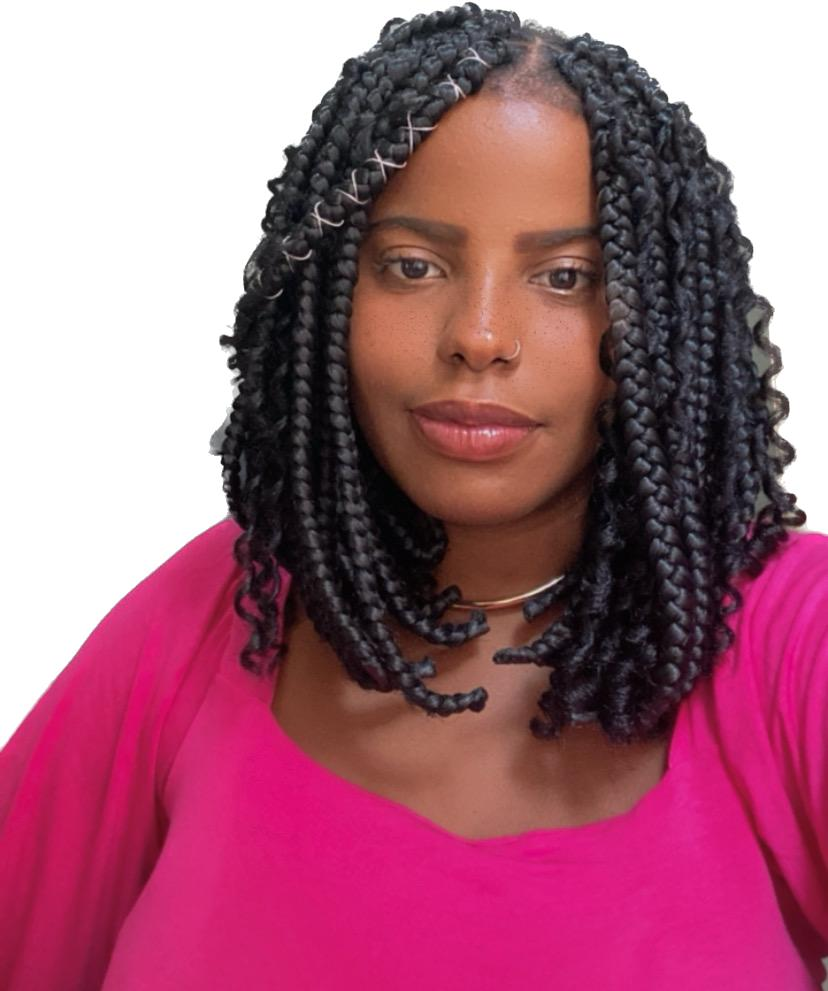
\includegraphics[width=2cm]{Helena.jpg}
		\end{wrapfigure}
		Helena Beatriz Jesus Gomes é licenciada 
		em Matemática pela Universidade Federal da Bahia (UFBA). 
		É membro do Grupo de Estudos e Pesquisas em Didática e Educação Matemática Inclusiva 
		(UFCG). Sua área de interesse é Educação Matemática 
		Inclusiva e Tecnologia no Ensino de Matemática.		
\end{minipage}	
\begin{minipage}{10cm}
	\vspace{0.3cm}
	\begin{wrapfigure}{L}{1.5cm}
		\vspace{-10pt}
		\centering
		
\includegraphics[width=2cm]{Taise.jpg}
	\end{wrapfigure}
	Taíse Lara de Souza Jorge é licenciada em Matemática pela UFBA 
	e mestranda em Educação pela UFFS. Realiza pesquisa na área de Mediação
	Pedagógica e Alfabetização Matemática sob a perspectiva do Numeramento, 
	amparada na Educação Crítica e Educação Matemática Crítica. 
\end{minipage}
	
\end{center}



\newpage

\pagestyle{empty}
\pagecolor{olivalight}
~
\vfill
\begin{center}
	\includegraphics[width=9cm]{Logos_contracapa_Hipátia_2.jpeg}

	\vspace{4cm}

	
\includegraphics[width=4cm]{QR.png}
	
	Link para o \emph{site} da
	
	Revista de Matemática Hipátia

\end{center}

\vfill
\newpage
\AddToHookNext{shipout/background}
 {%
  \put(0,-\paperheight)
{\begin{tikzpicture}
\meanderbox{8}{13}{0.888}
\end{tikzpicture}}
}

~\\[4cm]
\begin{center}
	
\includegraphics[width=10cm]{Hipatiaazul.png}
\end{center}


\end{document}